\documentclass[border=5mm]
{standalone}
%\usepackage{amsmath}
\usepackage{xcolor,times}
\usepackage{pgfplots}
\usepgfplotslibrary{groupplots}
\usetikzlibrary{patterns}
\usepackage{tikz}
\begin{document}
%\pgfplotsset{width=18cm,height=10cm}
% This file was created with tikzplotlib v0.10.1.
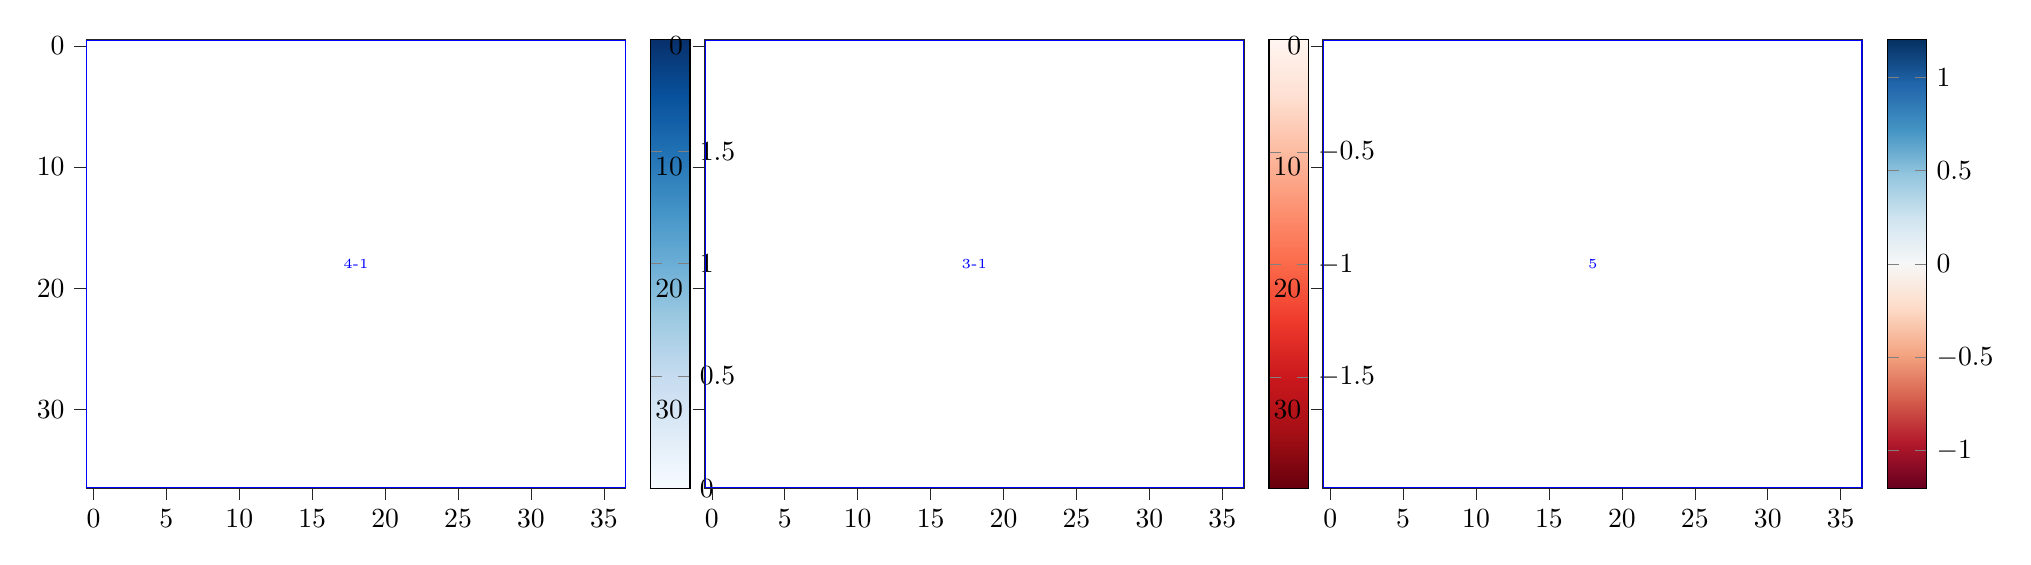
\begin{tikzpicture}

\definecolor{darkslategray38}{RGB}{38,38,38}
\definecolor{lightgray204}{RGB}{204,204,204}

\begin{groupplot}[group style={group size=3 by 1}]
\nextgroupplot[
axis line style={darkslategray38},
colorbar,
colorbar style={ylabel={}},
colormap={mymap}{[1pt]
  rgb(0pt)=(0.968627450980392,0.984313725490196,1);
  rgb(1pt)=(0.870588235294118,0.92156862745098,0.968627450980392);
  rgb(2pt)=(0.776470588235294,0.858823529411765,0.937254901960784);
  rgb(3pt)=(0.619607843137255,0.792156862745098,0.882352941176471);
  rgb(4pt)=(0.419607843137255,0.682352941176471,0.83921568627451);
  rgb(5pt)=(0.258823529411765,0.572549019607843,0.776470588235294);
  rgb(6pt)=(0.129411764705882,0.443137254901961,0.709803921568627);
  rgb(7pt)=(0.0313725490196078,0.317647058823529,0.611764705882353);
  rgb(8pt)=(0.0313725490196078,0.188235294117647,0.419607843137255)
},
point meta max=1.99854334537461,
point meta min=0.000248569579851865,
tick align=outside,
tick pos=left,
x grid style={lightgray204},
xmin=-0.5, xmax=36.5,
xtick style={color=darkslategray38},
y dir=reverse,
y grid style={lightgray204},
ymin=-0.5, ymax=36.5,
ytick style={color=darkslategray38}
]
\addplot graphics [includegraphics cmd=\pgfimage,xmin=-0.5, xmax=36.5, ymin=36.5, ymax=-0.5] {4-1};

\nextgroupplot[
axis line style={darkslategray38},
colorbar,
colorbar style={ylabel={}},
colormap={mymap}{[1pt]
  rgb(0pt)=(0.403921568627451,0,0.0509803921568627);
  rgb(1pt)=(0.647058823529412,0.0588235294117647,0.0823529411764706);
  rgb(2pt)=(0.796078431372549,0.0941176470588235,0.113725490196078);
  rgb(3pt)=(0.937254901960784,0.231372549019608,0.172549019607843);
  rgb(4pt)=(0.984313725490196,0.415686274509804,0.290196078431373);
  rgb(5pt)=(0.988235294117647,0.572549019607843,0.447058823529412);
  rgb(6pt)=(0.988235294117647,0.733333333333333,0.631372549019608);
  rgb(7pt)=(0.996078431372549,0.87843137254902,0.823529411764706);
  rgb(8pt)=(1,0.96078431372549,0.941176470588235)
},
point meta max=-0.000799789190698674,
point meta min=-1.99445938463059,
tick align=outside,
tick pos=left,
x grid style={lightgray204},
xmin=-0.5, xmax=36.5,
xtick style={color=darkslategray38},
y dir=reverse,
y grid style={lightgray204},
ymin=-0.5, ymax=36.5,
ytick style={color=darkslategray38}
]
\addplot graphics [includegraphics cmd=\pgfimage,xmin=-0.5, xmax=36.5, ymin=36.5, ymax=-0.5] {3-1};

\nextgroupplot[
axis line style={darkslategray38},
colorbar,
colorbar style={ylabel={}},
colormap={mymap}{[1pt]
  rgb(0pt)=(0.403921568627451,0,0.12156862745098);
  rgb(1pt)=(0.698039215686274,0.0941176470588235,0.168627450980392);
  rgb(2pt)=(0.83921568627451,0.376470588235294,0.301960784313725);
  rgb(3pt)=(0.956862745098039,0.647058823529412,0.509803921568627);
  rgb(4pt)=(0.992156862745098,0.858823529411765,0.780392156862745);
  rgb(5pt)=(0.968627450980392,0.968627450980392,0.968627450980392);
  rgb(6pt)=(0.819607843137255,0.898039215686275,0.941176470588235);
  rgb(7pt)=(0.572549019607843,0.772549019607843,0.870588235294118);
  rgb(8pt)=(0.262745098039216,0.576470588235294,0.764705882352941);
  rgb(9pt)=(0.129411764705882,0.4,0.674509803921569);
  rgb(10pt)=(0.0196078431372549,0.188235294117647,0.380392156862745)
},
point meta max=1.2,
point meta min=-1.2,
tick align=outside,
tick pos=left,
x grid style={lightgray204},
xmin=-0.5, xmax=36.5,
xtick style={color=darkslategray38},
y dir=reverse,
y grid style={lightgray204},
ymin=-0.5, ymax=36.5,
ytick style={color=darkslategray38}
]
\addplot graphics [includegraphics cmd=\pgfimage,xmin=-0.5, xmax=36.5, ymin=36.5, ymax=-0.5] {5};
\end{groupplot}

\end{tikzpicture}


\end{document} 